\newpage
%
% Návrh
%
\ifthenelse {\boolean{bachelor}}
{
	%\section{Design}
	\section{Návrh}
}
{
	%\chapter{Design}
	\chapter{Návrh}
}
\label{section:design}

%
% Uchovávanie textov v databázach
%
\ifthenelse {\boolean{bachelor}}
{
	%\subsection{Subsection}
	\subsection{Uchovávanie textov v databázach}
}
{
	%\section{Subsection}
	\section{Uchovávanie textov v databázach}
}
\label{subsection:persisting_texts_in_db}
Text je špecifický údajový model s variabilnou štruktúrou. Ak chceme efektívne ukladať texty v databázach, je nutné aby sme použili databázu, ktorá je tomu prispôsobená, pri ktorej nebudeme zbytočne čerpať pamäť a takisto bude jednoduché narábať s dátami. To znamená bezproblémové ukladanie, získavanie, vyhľadávanie a spracovanie textov na úrovni databázy. V nasledujúcich kapitolách sa pozrieme, aké typy databáz existujú a aké možnosti z pohľadu ukladania textov ponúkajú.

%
% Relačné databázy
%
\ifthenelse {\boolean{bachelor}}
{
	%\subsection{Subsection}
	\subsubsection{Relačné databázy}
}
{
	%\section{Subsection}
	\subsection{Relačné databázy}
}
\label{subsubsection:relation_dbs}
Relačné databázy boli dlhé roky populárnou a finančné nenáročnou voľbou pri tvorbe veľkých podnikateľských aplikácií. Momentálne sú používané vo väčšine súčasných aplikácií a pracujú spoľahlivo pri obmedzenom množstve dát~\cite{MongoDBvsMySQL2015}. Problém s relačným modelom relačných databáz nastáva, keď vzniká potreba aplikácie s obrovským množstvom dát. Menovite rozšíriteľnosť (angl. scalability) sa stáva najväčším problémom relačných databáz~\cite{NoSQLDBvsRealtionDB}.

Tento typ databáz oplýva veľkou úrovňou jednotvárnosti, ukladá dáta v tabuľkách zložených z riadov a stĺpcov. Každý záznam (riadok) v tabuľke predstavuje zjednodušený objekt alebo vzťah z reálneho života. Výhodou relačných databáz je možnosť jednoduchého vytvorenia prispôsobeného pohľadu na dáta~\cite{Maier}.

%
% Textové databázy
%
\ifthenelse {\boolean{bachelor}}
{
	%\subsection{Subsection}
	\subsubsection{Textové databázy}
}
{
	%\section{Subsection}
	\subsection{Textové databázy}
}
\label{subsubsection:text_dbs}
S rozmachom variácie dát v posledných rokoch sa začali objavovať a vznikať nerelačné databázy, aby pokryli požiadavky na nové aplikácie. Textové databázy sú druhom nerelačných databáz.

Textové databázy ukladajú dáta vo forme dokumentov, vďaka čomu ponúkajú vysoký výkon a horizontálnu rozšíriteľnosť~\cite{NoSQLDBvsRealtionDB}. Uložené dokumenty môžu nadobúdať rôzne typy, ako napríklad JSON, BSON, XML a BLOB, ktoré poskytujú veľkú flexibilnosť pre dáta. Každý záznam v takejto databáze preto môže mať inú štruktúru, napríklad počet alebo typ polí, čo šetrí úložným priestorom, keďže neobsahuje nepotrebné prázdne polia~\cite{NoSQLDBvsRealtionDB}.

Dokumenty v databáze sú referencované kľúčom, ktorý môže byť string, cesta, ale dokonca aj dokument~\cite{NoSQLDBvsRealtionDB}. Majú dynamickú schému, čo umožňuje vytvárať záznamy bez toho, aby bolo potrebné predtým definovať štruktúru. Uľahčujú zmenu štruktúry záznamov jednoduchým pridaním, odstránením alebo zmenením typu poľa. Vďaka svojej štruktúre sú dokumenty ľahko namapovateľné na objekty z objektovo-orientovaných programovacích jazykov a odstraňujú tým potrebu pre použitie objektovo-relačnej mapovacej vrstvy.
\\

Primárne využitie týchto databáz je v aplikáciách, ktoré potrebujú ukladať dáta, ktorých štruktúra je vopred neznáma alebo sa mení. Predstaviteľmi sú napríklad \textit{MongoDB} alebo \textit{CouchDB} databázy.

%
% MongoDB
%
\ifthenelse {\boolean{bachelor}}
{
	%\subsection{Subsection}
	\paragraph{MongoDB}
}
{
	\%section{Subsection}
	\subsubsection{MongoDB}
}
\label{subsection:mongodb}
MongoDB\footnote{www.mongodb.org} je dokumentová nerelačná databáza vytvorená v C++ spustená v roku 2009~\cite{NoSQLDBvsRealtionDB}. Ukladá dáta v dokumentoch vo formáte BSON (Binary JSON), ktorých štruktúra sa môže meniť. Využíva dynamickú štruktúru schém, preto dokáže vytvárať záznamy bez preddefinovanej štruktúry dát, lebo štruktúra sa vytvára za behu, pričom môže byť veľmi jednoducho pozmenená pridaním, odstránením alebo zmenou typu polia dokumentu určujúceho štruktúru. Umožňuje jednoduché ukladanie dát s hierarchickými vzťahmi alebo komplexnejších štruktúr, ako sú napríklad polia, listy alebo vnorené polia.

Vlastnosti ako chybová tolerancia, perzistencia a konzistencia dát sú súčasťou MongoDB. Oproti klasickým dokumentovým databázam ponúka aj vymoženosti, ako agregácia, ad hoc dopyty, indexovanie, a pod. Taktiež má svoj vlastný plnohodnotný dopytovací jazyk \textit{mongo query language}~\cite{NoSQLDBvsRealtionDB}.

Prvky poskytované databázou MongoDB sú prvky zahrnuté v relačných databázach rozšírené o ďalšiu funkcionalitu. Porovnanie poskytovaných prvkov je v tabuľke~\fullref{table:features_of_mongodb}. 

\begin{table}[H]
	\centering
	\caption{Prvky poskytované MongoDB}
	\label{table:features_of_mongodb}
	\begin{tabular}{|l|l|l|}
		\hline
		& \textbf{MySQL} & \textbf{MongoDB} \\ \hline
		Bohatý dátový model & Nie & Áno \\ \hline
		Dynamická štruktúra & Nie & Áno \\ \hline
		Dátové typy & Áno & Áno \\ \hline
		Lokálnosť dát & Nie & Áno \\ \hline
		Aktualizovanie polí & Áno & Áno \\ \hline
		Ľahké pre programátorov & Nie & Áno \\ \hline
		Komplexné transakcie & Áno & Nie \\ \hline
		Audit & Áno & Áno \\ \hline
		Auto-sharding & Nie & Áno \\ \hline
	\end{tabular}
\end{table}

Bohatý dátový model (angl. Rich Data Model) znamená, že dátový model poskytuje veľa funkcionality. Princípom dynamickej štruktúry (angl. Dynamic Structure) je jednoduchá zmena štruktúru, pričom nemusí byť vôbec zadefinovaná a každý záznam môže mať odlišnú štruktúru. Lokálnosť dát (angl. Data Locality) znamená uchovávanie súvisiacich dát pokope. Aktualizovanie polí umožňuje vykonávať nad poliami operácie, ako sú inkrementácia podľa špecifikovaného množstva, vynásobenie hodnotou, premenovanie, aktualizácia iba ak je hodnota väčšia alebo menšia ako špecifická hodnota a ďalšie. Audit (angl. Auditing) je funkcionalita, ktorá umožňuje administrátorom a používateľom sledovať aktivity systému.
Auto-sharding pri náraste dát, aby sa zabránilo poklesu priepustnosti operácií čítania a zapisovania, ukladá dáta automaticky na viacero strojov.

MongoDB má vlastnú konvenciu názvov svojich častí. Tie sa v niektorých prípadoch líšia s názvami relačných databáz. Rozdiely sú zobrazene v tabuľke~\fullref{table:names_of_mongodb}. Za zástupcu relačných databáz bola vybraná MySQL databáza. 

\begin{table}[H]
	\centering
	\caption{Porovnanie používaných pojmov~\cite{MongoDBvsMySQL2015}}
	\label{table:names_of_mongodb}
	\begin{tabular}{|l|l|}
		\hline
		\textbf{MySQL} & \textbf{MongoDB} \\ \hline
		Databáza & Databáza \\ \hline
		Tabuľka & Kolekcia \\ \hline
		Index & Index \\ \hline
		Riadok & BSON dokument \\ \hline
		Stĺpec & BSON pole (angl. field) \\ \hline
		Spojenie & Vnorené dokumenty a prepojenie \\ \hline
		Primárny kľúč & Primárny kľúč \\ \hline
		Zoskupenie & Agregácia \\ \hline
	\end{tabular}
\end{table}

%
% Ostatné databázové systémy
%
\ifthenelse {\boolean{bachelor}}
{
	%\subsection{Subsection}
	\subsubsection{Ostatné databázové systémy}
}
{
	\%section{Subsection}
	\subsection{Ostatné databázové systémy}
}
\label{subsection:types_of_norelation_dbs}
Okrem relačných a textových dokumentov existuje ešte niekoľko druhov databáz. V nasledujúcich častiach si priblížime niektoré z nerelačných databáz.

%
% Kľúč - hodnota databázy
%
\ifthenelse {\boolean{bachelor}}
{
	%\subsection{Subsection}
	\paragraph{Kľúč - hodnota databázy}
}
{
	\%section{Subsection}
	\subsubsection{Kľúč - hodnota databázy}
}
\label{subsubsection:key_value_db}
Nerelačné databázy typu kľúč - hodnota sú v svojej podstate celkom jednoduché, ale zároveň efektívne. Umožňujú používateľovi ukladať dáta ľubovoľne, kedže neobsahujú schémy. Uložené dáta sa skladajú z dvoch častí. Prvá časť je kľuč a druhá časť je hodnota~\cite{NoSQLDBvsRealtionDB}, pričom kľúč je samo-generujúci string a hodnota môže byť takmer čokoľvek, od string, JSON cez BLOB až po obrázok~\cite{MongoDBvsMySQL2015}.

Kľúč - hodnota databázy sú veľmi podobné hašovacím tabuľkám, kde kľúč je indexom do tabuľky, pomocou ktorého používateľ môže pristúpiť k hodnote daného kľúču. Tento typ databáz uprednostňuje rozšíriteľnosť pred konzistenciou. Ponúka vysokú konkurenčnosť (angl. concurrency), rýchle vyhľadávanie a schopnosť uloženia veľkého množstva dát za cenu spojovacích a agregačných operácií. Taktiež je veľmi náročné vytvoriť ľubovoľný pohľad na dáta z dôvodu chýbajúcej schémy~\cite{NoSQLDBvsRealtionDB}.

Najznámejšími predstaviteľmi tohto typu databáz sú \textit{Amazon DynamoDB} a \textit{RIAK}.

%
% Stĺpcové databázy
%
\ifthenelse {\boolean{bachelor}}
{
	%\subsection{Subsection}
	\paragraph{Stĺpcové databázy}
}
{
	\%section{Subsection}
	\subsubsection{Stĺpcové databázy}
}
\label{subsubsection:column_db}
Stĺpcové databázy musia mať preddefinovanú schému, v ktorej sú jednotlivé bunky záznamov zoskupené do kolekcie stĺpcov~\cite{MongoDBvsMySQL2015}. Dáta nie sú ukladané do tabuliek, ale do masívne distribuovaných architektúr, s hlavným zámerom, aby agregácia dát mohla prebehnúť veľmi rýchlo s redukovaním I/O aktivity.

Tento typ databáz taktiež poskytuje veľkú rozšíriteľnosť v ukladaní dát.

Najvhodnejšie je využívať stĺpcové databázy v analytických aplikáciách alebo aplikáciách, ktoré získavajú dáta pomocou metódy \textit{data mining}~\cite{NoSQLDBvsRealtionDB}.

%
% Grafové databázy
%
\ifthenelse {\boolean{bachelor}}
{
	%\subsection{Subsection}
	\paragraph{Grafové databázy}
}
{
	\%section{Subsection}
	\subsubsection{grafové databázy}
}
\label{subsubsection:graph_db}
Grafové databázy su špeciálny typ databáz, v ktorých sú dáta uložené vo forme grafu. Graf pozostáva z vrcholov a hrán, pričom vrcholy predstavujú objekty a hrany reprezentujú vzťahy medzi nimi. Každý vrchol okrem iného obsahuje aj ukazovateľ na priľahlé vrcholy, čo umožňuje prechádzať obrovské množstvo dát rýchlejšie ako v relačných databázach~\cite{NoSQLDBvsRealtionDB}.

Údaje sa ukladajú v polo-štruktúrovanej forme, kde je kladený hlavný dôraz na prepojenia medzi dátami. Grafové databázy spĺňajú vlastnosť ACID a sú veľmi vhodné pre biometrické aplikácie alebo aplikácie sociálnych sietí. Hlavným predstaviteľom grafových databáz je \textit{Neo4j}~\cite{NoSQLDBvsRealtionDB}.

%
% Objektovo orientované databázy
%
\ifthenelse {\boolean{bachelor}}
{
	%\subsection{Subsection}
	\paragraph{Objektovo orientované databázy}
}
{
	\%section{Subsection}
	\subsubsection{Objektovo orientované databázy databázy}
}
\label{subsubsection:object_oriented_db}
Objektovo orientované databázy ukladajú dáta vo forme objektov, rovnako ako sú údaje reprezentované v objektoch v objektovo orientovaných programovacích jazykoch (OOP). Tieto databázy podporujú všetky vymoženosti OOP, ako enkapsulácia, polymorfizmus, ale aj dedenie. Objektovo orientované databázy robia moderný vývoj softvéru jednoduchším~\cite{NoSQLDBvsRealtionDB}.

%
% Zhrnutie
%
\ifthenelse {\boolean{bachelor}}
{
	%\subsection{Subsection}
	\subsubsection{Zhrnutie}
}
{
	%\section{Subsection}
	\subsection{Zhrnutie}
}
NOSQL databáza narozdiel do RDBMS modelu (Relation Data Base Management System) je
navrhnutá, aby bola jednoducho rozšíriteľná so zväčšovaním sa. Väčšina NOSQL databáz odstránila niektoré nepotrebné prvky RDBMS modelov, čím sa stali podstatne ľahšími a efektívnejšími ako ich náprotivok RDBMS systémy. Toto na druhej strane spôsobilo, že NOSQL model negarantuje vlastnosti ACID (Atomicity, Consistency, Isolation, Durability), ale naopak garantuje vlastnosti BASE (Basically Available, Soft state, Eventula Consistency)~\cite{NoSQLDBvsRealtionDB}.

Nerelačné databázy neukladajú údaje v tabuľkách a nemajú fixnú schému. Tieto vlastnosti im umožňujú jednoducho spracovávať neštruktúrované dáta, ako sú dokumenty, e-maily a mnoho ďalších~\cite{MongoDBvsMySQL2015}. Preto majú čím ďalej, tým viac využití.

Existuje hneď niekoľko prípadov, kedy je lepšie použiť nerelačnú databázu namiesto relačnej databázy. Keď je potrebné, aby aplikácia dokázala spracovávať rôzne typy a tvary dát alebo pri potrebe spravovať aplikáciu efektívnejšie pri rozširovaní, je rozhodne výhodnejšie použiť nerelačnú databázu. Niektoré databázy, ako napríklad textová databáza MongoDB uľahčuje vývoj aplikácií, keďže jeho dokumentová štruktúra dát je jednoducho namapovateľná na moderné, objektovo-orientované programovacie jazyky a tým pádom nie je potreba využívať komplexnú objektovo-relačnú mapovaciu vrstvu, ktorá je nutná pri použití relačných databáz na prevod objektov z programovacie jazyka na perzistentné objekty v databáze. Všeobecne je omnoho ľahšie rozšíriť schému / model nerelačnej databázy ako rozširovať schému relačnej databázy.

Potrebujeme ukladať v databáze texty a informácie o nich. Počet viet, slov, vzťahov je pre každý text odlišný a preto nedokážeme vopred definovať efektívnu schému na ukladanie týchto dát. Textové databázy, so svojou dynamickou a ľahko upraviteľnou štruktúrou, sú na tento účel ideálne, pričom ukladanie textov v tabuľkách by bolo náročne, navyše relačné databázy nemajú default podporované vyhľadávania v štruktúrach ako text. MongoDB (viď.~\fullref{subsection:mongodb}) je vyspelá, textová databáza zahrňajúca všetku funkcionalitu, ktorú potrebujeme navyše rozšírenú o veľa vymožeností.

%
% Návrh uchovávania textov v databázach
%
\ifthenelse {\boolean{bachelor}}
{
	%\subsection{Subsection}
	\subsection{Návrh uchovávania textov v databázach}
}
{
	%\section{Subsection}
	\section{Návrh uchovávania textov v databázach}
}
\label{subsection:our_design_persisting_data}
Dáta budeme ukladať v dokumentovej databáze MongoDB. Keďže spracovávané dáta sa dajú rozdeliť do troch kategórií, budeme využívať primárne tri databázové kolekcie na ich ukladanie. Sú to:

\begin{my_itemize}
	\myitem sentences,
	\myitem rules,
	\myitem texts.
\end{my_itemize}
	
Pri návrhu sme vychádzali z princípu čo najjednoduchších kolekcií, ktoré budu obsahovať iba relevantné informácie.
V nasledujúcich častiach ich opíšeme bližšie aj s názornými ukážkami.

%
% Kolekcia texts
%
\ifthenelse {\boolean{bachelor}}
{
	%\subsection{Subsection}
	\subsubsection{Kolekcia texts}
}
{
	%\section{Subsection}
	\subsection{Kolekcia texts}
}
V kolekcií \textit{texts} sa ukladajú celé texty, ktoré sú spracovávané. 

Kolekcia obsahuje iba jedno pole textového typu slúžiace na uloženie textu v pôvodnom tvare. Štruktúra uložených dát v kolekcií \textit{texts} je zobrazená na obrázku~\fullref{fig:texts_collection_structure}.

\begin{figure}[H]
	\begin{center}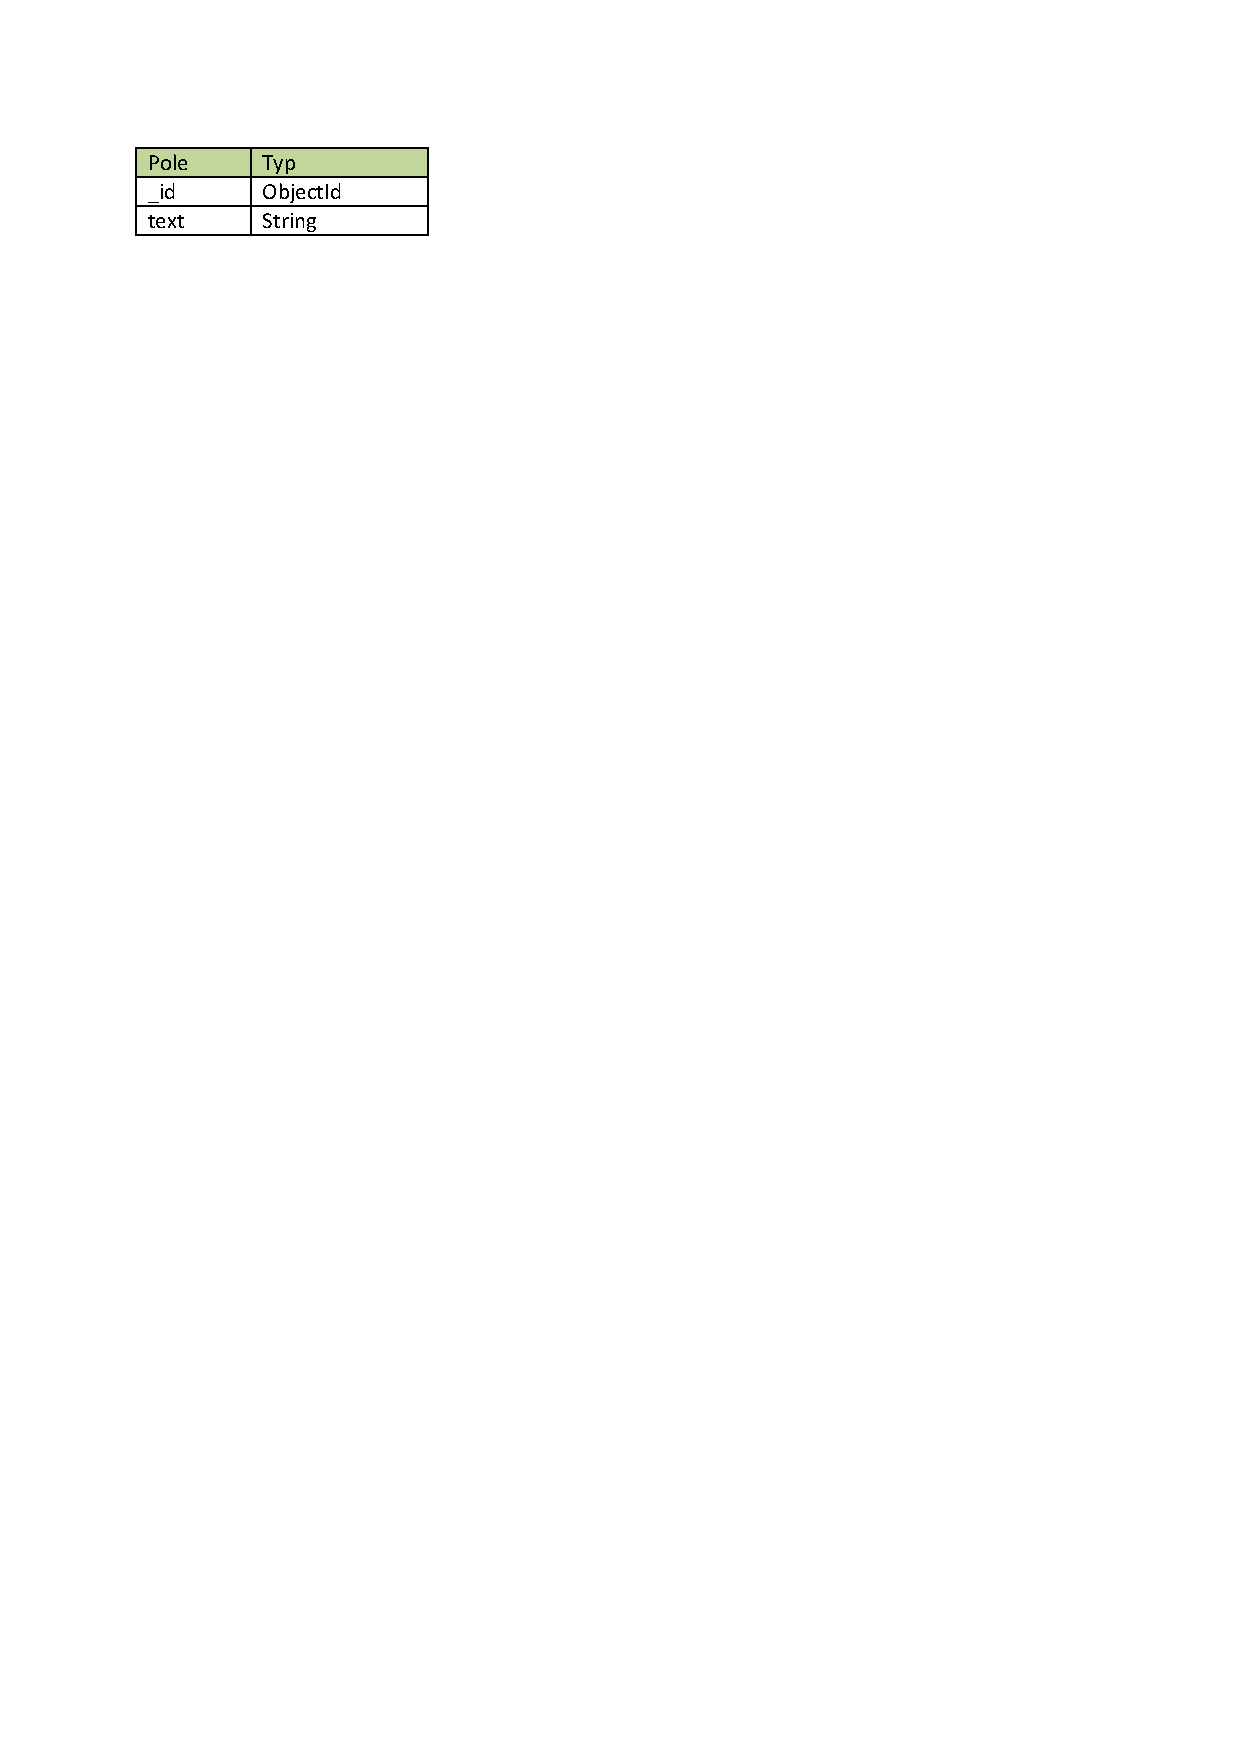
\includegraphics[scale=0.60]{texts_collection}\end{center}
	\caption[Štruktúra kolekcie texts]{Štruktúra kolekcie texts}\label{fig:texts_collection_structure}
\end{figure}

%
% Kolekcia sentences
%
\ifthenelse {\boolean{bachelor}}
{
	%\subsection{Subsection}
	\subsubsection{Kolekcia sentences}
}
{
	%\section{Subsection}
	\subsection{Kolekcia sentences}
}
V ďalšej kolekcii \textit{sentences} ukladáme spracovávané vety a vytvorené poznámky z týchto viet, pričom vety sa odkazujú na texty, z ktorých pochádzajú v kolekcií \textit{texts}. Umožní nám to jednoducho zistiť, v akom texte sa daná veta nachádzala.

Dáta sú uložené v dokumentoch, ktoré obsahujú tri polia. Jedno, textové, určené na uchovanie pôvodného znenia vety, druhé tiež textové na uchovanie novo vytvorenej vety po spracovaní vety uloženej v prvom poli a tretie pole, ktoré bude odkazovať na záznam v kolekcii \textit{texts}. Štruktúra dát v tejto kolekcií je načrtnutá na obrázku~\fullref{fig:sentences_collection_structure}.

\begin{figure}[H]
	\begin{center}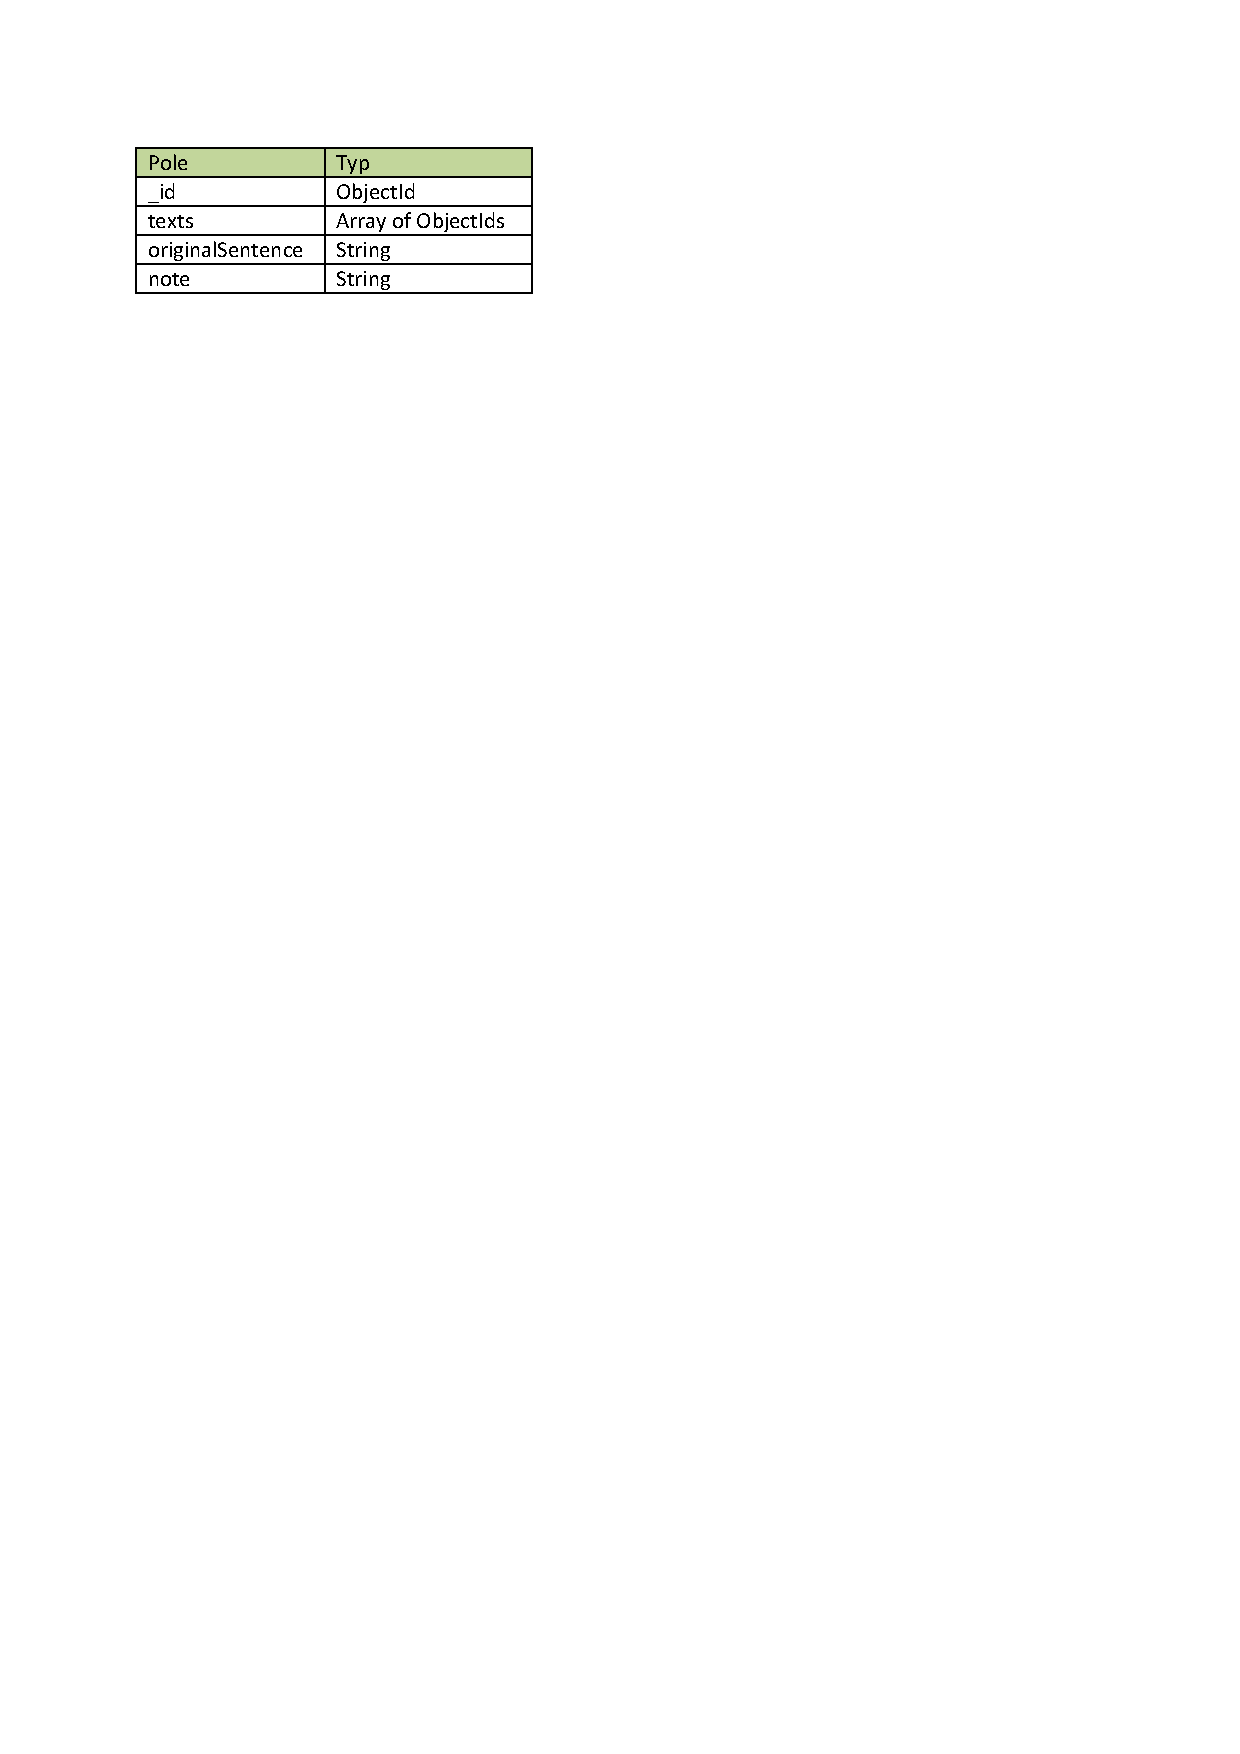
\includegraphics[scale=0.60]{sentences_collection}\end{center}
	\caption[Štruktúra kolekcie sentences]{Štruktúra kolekcie sentences}\label{fig:sentences_collection_structure}
\end{figure}

%
% Kolekcia rules
%
\ifthenelse {\boolean{bachelor}}
{
	%\subsection{Subsection}
	\subsubsection{Kolekcia rules}
}
{
	%\section{Subsection}
	\subsection{Kolekcia rules}
}
V poslednej kolekcii pomenovanej \textit{rules} sa ukladajú pravidla na spracovávanie viet, ktoré sa odkazujú na vety v kolekcii \textit{sentences}, ktoré boli podľa daného pravidla spracované. Ukladaním viet a pravidiel na ich spracovanie do separátnych kolekcií zabránime duplikovaniu dát a zrýchlime vyhľadávanie. Referencia do kolekcie \textit{sentences} nám poskytuje možnosť jednoduchého a rýchleho vyhľadanie viet, na ktoré bolo konkrétne pravidlo aplikované a aký bol výstup aplikovania tohto pravidla.

Pravidlo sa skladá hlavne z dvoch častí. Zoznam závislostí pôvodnej vety a zoznam závislostí zjednodušenej vety. Práve závislosti z druhého menovaného zoznamu sa aplikujú na spracovávanú vetu s cieľom zjednodušiť ju.

Každý záznam v tejto kolekcií obsahuje pole celých čísel určujúcich pozície slov, za ktorými je vo vytvorenej zjednodušenej vete ukončenie vety. V prípade jednoduchých viet to bude posledné slovo vety, ale pri súvetiach to môže byť viacero slov na ľubovolných miestach vety. Pre jednoduchú vetu \textit{,,The president of the Czech Republic is Miloš Zeman.''} bude toto pole obsahovať jednú hodnotu 3, keďže zjednodušená veta bude v tvare \textit{,,President is Zeman.''}. Pre zloženú vetu v tvare \textit{,,Czech Republic has no sea; its neighbour countries are Germany, Austria, Slovakia and Poland.''} bude spomínané pole obsahovať dve hodnoty, keďže táto veta sa skladá z dvoch. Prvá obsahujúca informáciu o mori a druhá s informáciou o susedných štátoch, a tak sa aj spracuje pri zjednodušovaní.

Okrem poľa určujúceho konce viet, bude každý záznam obsahovať dva hlavné zoznamy závislostí. Prvý zoznam bude pozostávať zo závislostí pôvodnej vety a druhý zoznam bude zložený zo závislostí zjednodušenej vety. Zoznamy majú nasledujúcu štruktúru. Obsahujú dokumenty. Tieto dokumenty majú názov vzťahu závislosti a ich zoznam, pričom sa párujú práve podľa názvu. Tento vnorený zoznam obsahuje už konkrétne závislosti. Každá závislosť uložená v databáze sa skladá z nadradeného tokenu (angl. governor), podradeného tokenu (angl. dependent) a pozície tejto závislosti medzi všetkými závislosťami vety. Tokeny sú dokumenty skladajúce sa z dvoch polí, jedno textové, obsahujúce skratku POS značky a druhé číselne, obsahujúce pozíciu slova vo vete, ku ktorému sa daný token viaže.

Celá štruktúra dát v kolekcii \textit{rules} sa dá vyjadriť diagramom~\fullref{fig:rules_collection_structure}.

\begin{figure}[H]
	\begin{center}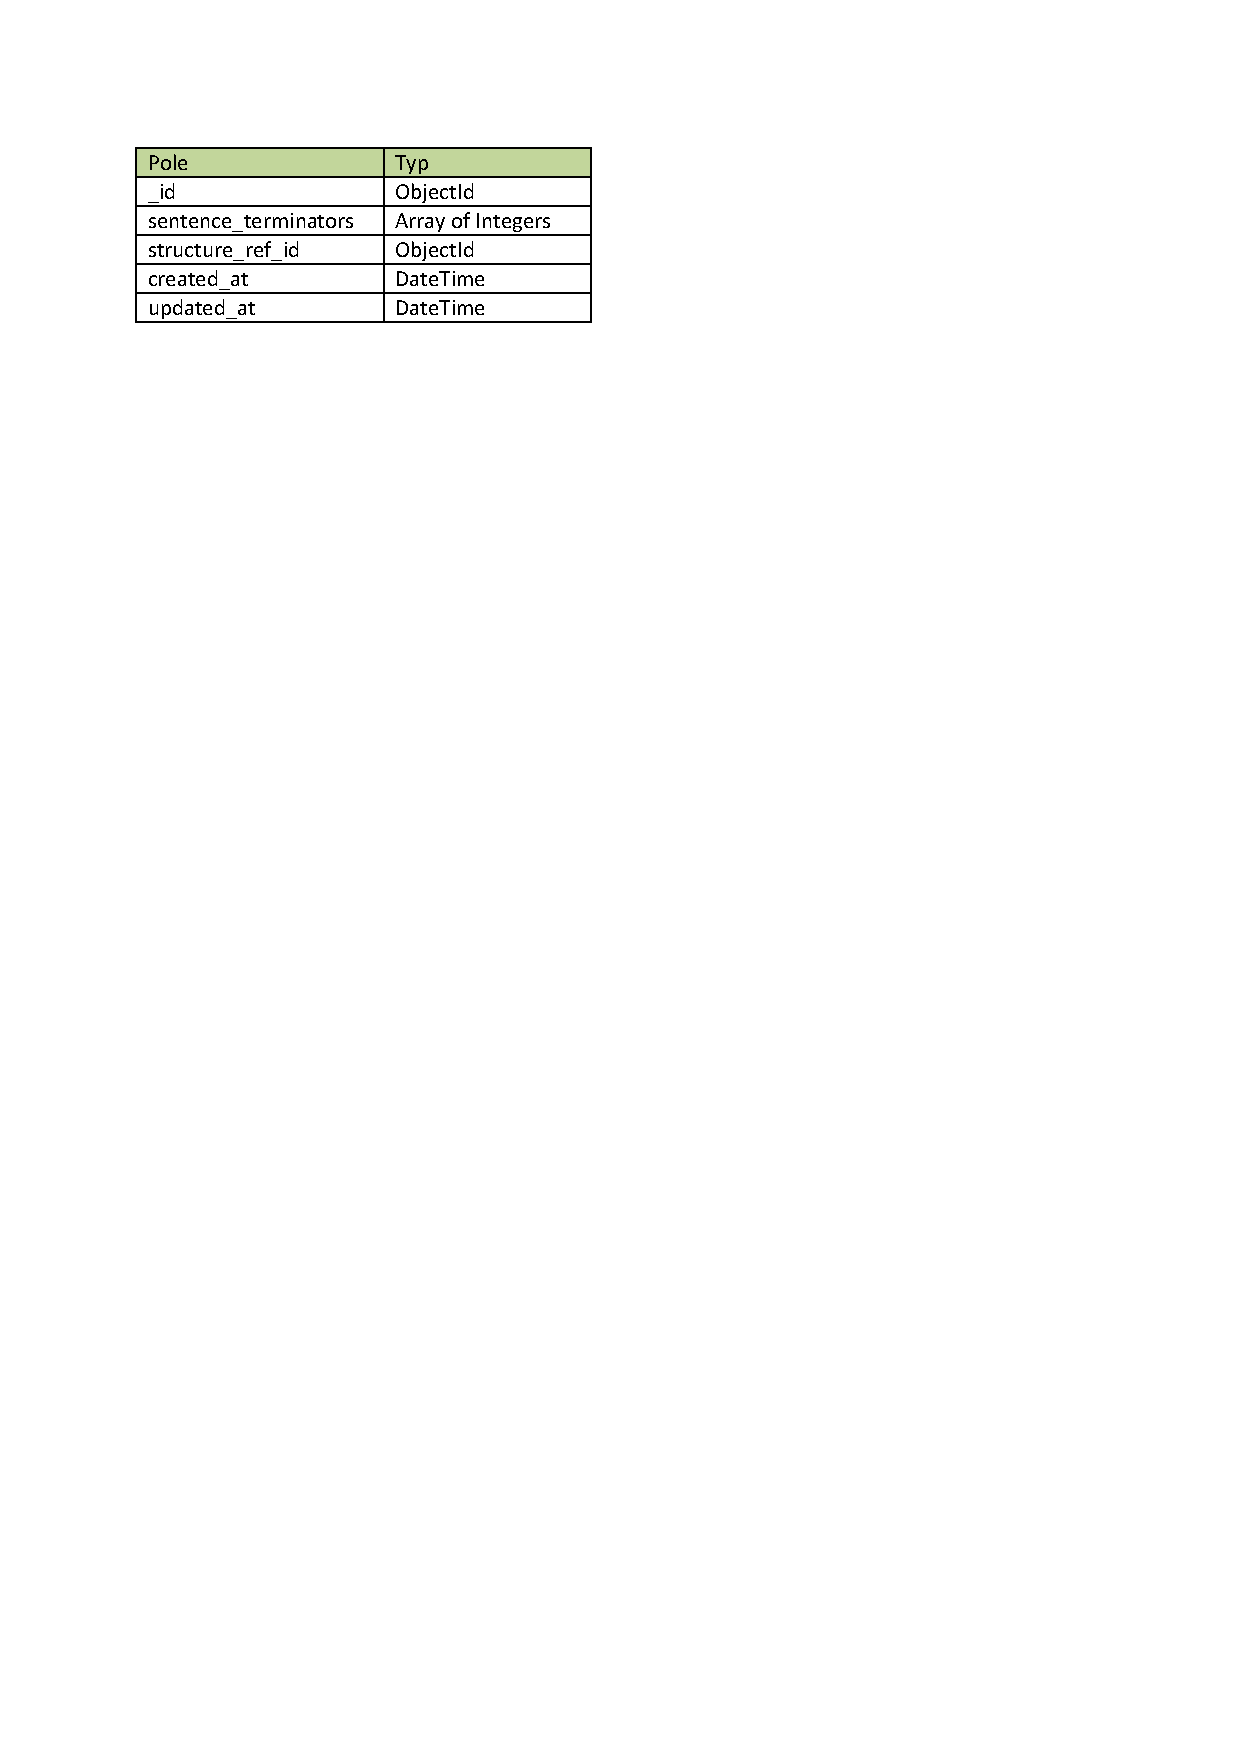
\includegraphics[scale=0.45]{rules_collection}\end{center}
	\caption[Štruktúra kolekcie rules]{Štruktúra kolekcie rules}\label{fig:rules_collection_structure}
\end{figure}

Dáta sú v MongoDB databáze uložené v binárnom JSON formáte. Na ukážke~\fullref{code:collection_rules_data_example} je zobrazená časť uložených údajov o pôvodnej vete. Ukážka celého záznamu pre vetu ,,The president of the Czech Republic is Milos Zeman.'' je priložená v prílohe~\fullref{appendix:db_entry_full_example}.
\\
\begin{lstlisting}[language = json, caption={Ukážka dát kolekcie rules}, label = {code:collection_rules_data_example}]
{  
	"originalDependencies" : [  
		{  
			"dependencyName" : "det",
			"dependencies" : [  
				{  
					"governor" : {  
						"pos" : "NN",
						"index" : 2
					},
					"dependent" : {  
						"pos" : "DT",
						"index" : 1
					},
					"position" : 0
				},
				{ ... }
			]
		}
	]
}
\end{lstlisting}


%
% Manažment dát
%
\ifthenelse {\boolean{bachelor}}
{
	%\subsection{Subsection}
	\subsection{Manažment dát}
}
{
	%\section{Subsection}
	\section{Manažment dát}
}
\label{subsection:data_management}
V nasledujúcich častiach si priblížime narábanie s dátami z databázy, ako vyhľadanie pravidla, jeho aplikovanie alebo vytvorenie pravidla, ak žiadne nebolo vyhľadané.

%
% Vyhľadávanie pravidla
%
\ifthenelse {\boolean{bachelor}}
{
	%\subsection{Subsection}
	\subsubsection{Vyhľadávanie pravidla}
}
{
	%\section{Subsection}
	\subsection{Vyhľadávanie pravidla}
}
\label{subsubsection:rule_lookup}
Pred spracovaním vety sa vyhľadá pravidlo v databáze vhodné na jej zjednodušenie. Pri vyhľadávaní sa berie do úvahy viacero podmienok.

Spracovávaná veta, pre ktorú hľadáme pravidlo, musí mať rovnaký počet záznamov v \textit{zozname závislosti pôvodnej vety} a zároveň musia byť napárované práve všetky názvy vzťahov v závislostiach v tomto zozname.

Pri použití týchto podmienok vieme rýchlo vyhľadať pravidlo, ktoré súvisí s podobnou vetou. Avšak, môže nastať situácia, kedy je pre spracovávanú vetu vhodných viacero pravidiel. Vtedy sa rozhoduje podľa zhody pôvodných viet, ktoré vybrať. Vyberá sa, a následne aplikuje, to s najväčšou zhodou.

Určovanie najväčšej zhody má viacero krokov. Najskôr sa spočítavajú zhody POS značiek nadradených a podradených tokenov zvlášť a následne, indexy slov prislúchajúcich tokenom taktiež nezávisle od seba. Tým sa zisťuje, či spracovávaná veta obsahuje ľubovoľnú závislosť s rovnakou hodnotou POS značky alebo indexu či už nadradeného alebo podradeného tokenu. V druhom kroku sa určuje polovičná zhoda závislosti, teda či spracovávaná veta obsahuje zhody POS značiek a zároveň indexov slov v nadradenom tokene alebo v podradenom tokene. V poslednom, treťom sa zisťuje počet úplných zhôd závislostí, čo znamená zhoda POS značiek a indexov zároveň, v nadradenom a podradenom tokene zároveň. Tieto tri hodnoty sa na záver spočítajú a tým získame percentuálne ohodnotenie zhody viet.

Toto určovanie najväčšej zhody sa uskutoční pre každé vyhovujúce pravidlo a vyberie sa pravidlo s najväčšou zhodou. \\

Predpokladajme situáciu kedy spracovávame vetu ,,The local language is Czech language.'' a v databáze máme, okrem iného, uložené pravidlá pre vety ,,The local language is Czech language'' a ,,The Czech language is a Slavic language.''. Vtedy nastane, že pre spracovávanú vetu je vhodných viacero pravidiel. Keďže obe vety majú v \textit{zozname závislostí pôvodnej vety} práve 5 záznamov a tieto záznamy sa skladajú práve z množiny vzťahov \{det, amod, nsubj, cop, root\}, vyhľadanie pravidlá nám vráti minimálne tieto dve pravidlá. Po aplikovaní určenia najväčšej zhody týchto dvoch pravidiel a spracovávanou vetou, zistíme, že pravidlo prvej menovanej vety má so spracovávanou vetou cca. $99,99\%$ zhodu a pravidlo druhej vety má cca. $63,57\%$ zhodu. Aplikuje sa prvé pravidlo.

Ukážkový proces vyhľadania pravidla a určenie zhody je zobrazený na obrázku~\fullref{fig:rule_lookup}.

\begin{figure}[H]
	\begin{center}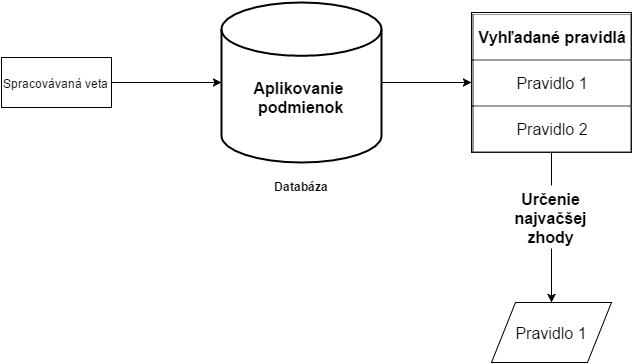
\includegraphics[scale=0.6]{rule_lookup}\end{center}
	\caption[Vyhľadanie pravidla]{Vyhľadanie pravidla}\label{fig:rule_lookup}
\end{figure}

%
% Vytváranie pravidla
%
\ifthenelse {\boolean{bachelor}}
{
	%\subsection{Subsection}
	\subsubsection{Vytváranie pravidla}
}
{
	%\section{Subsection}
	\subsection{Vytváranie pravidla}
}
\label{subsubsection:rule_creation}
Ak nám proces vyhľadania pravidla nevyhľadal žiadne pravidlo, znamená to, že sme doposiaľ nespracovávali takú istú alebo podobnú vetu. V tomto prípade použijeme náš parser, ktorý operuje nad staticky danou sadou pravidiel. Výstupom parseru bude zjednodušená veta, ktorej pravidlo sa následne uloží do databázy a pri ďalšom spracovávaní takej istej alebo podobnej vety sa toto pravidlo vyhľadá a aplikuje ak bude mať dostatočné veľkú zhodu.

Zo závislostí pôvodnej vety sa vytvorí \textit{zoznam závislostí pôvodnej vety}, zo závislostí zjednodušenej vety sa vytvorí \textit{zoznam závislostí zjednodušenej vety} a zo zjednodušenej vety sa určia konce viet. Tieto informácie sa spolu uložia do dokumentu (záznamu) do databázy ako \textbf{pravidlo}.

Na obrázku~\fullref{fig:rule_creation} je znázornený proces nevyhľadania pravidla, použitia parsera s následným uložením nového pravidla.

\begin{figure}[H]
	\begin{center}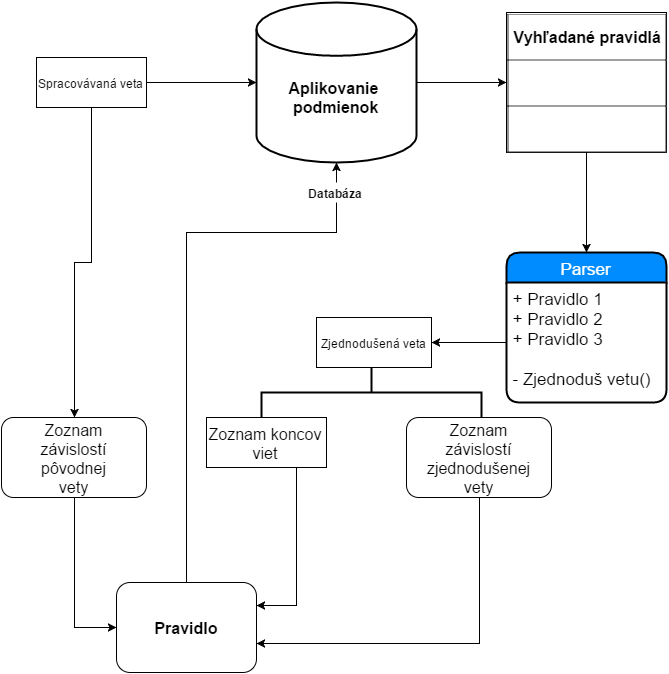
\includegraphics[scale=0.5]{rule_creation}\end{center}
	\caption[Vytvorenie pravidla]{Vytvorenie pravidla}\label{fig:rule_creation}
\end{figure}

%
% Aplikovanie pravidla
%
\ifthenelse {\boolean{bachelor}}
{
	%\subsection{Subsection}
	\subsubsection{Aplikovanie pravidla}
}
{
	%\section{Subsection}
	\subsection{Aplikovanie pravidla}
}
\label{subsubsection:rule_application}
Máme spracovávanú vetu a pravidlo na aplikovanie. Z princípu vyhľadávania pravidiel (viď.~\fullref{subsubsection:rule_lookup} pre podrobnosti) vieme, že spracovávaná veta obsahuje závislosti zo zoznamu závislostí pôvodnej vety a tým pádom obsahuje aj závislosti zo zoznamu závislostí zjednodušenej vety. 

Proces aplikovania pravidla prebieha nasledovne. Pre každú závislosť v zozname závislostí zjednodušenej vety, sa vyhľadá táto závislosť v spracovávanej vete. Z nájdenej závislosti sa zoberie slovo prislúchajúce podradenému tokenu a pridá sa do výslednej zjednodušenej vety na miesto svojho indexu. V prípade ak sa jedná o závislosť \textit{nominal subject}, zoberie sa aj slovo prislúchajúce nadradenému tokenu a taktiež sa pridá do výslednej vety. Po prejdení všetkých závislostí zo zoznamu sa urobia posledné úpravy zjednodušenej vety, ako kapitalizácia prvého písmena vety a rozdelenie vety na viacero viet, ak tak definovalo pravidlo.

Funkcia, ktorá bude aplikovať pravidlo na vetu s cieľom získania zjednodušenej vety bude vyzerať ako je naznačené v ukážke~\fullref{code:apply_rule_example}.
\\

\begin{lstlisting}[language = csharp, caption={Aplikovanie pravidla}, label = {code:apply_rule_example}]
// Funkcia aplikuje pravidlo na vetu a vrati zjednodusenu vetu
private Note ApplyRule(NotenizerSentence sentence, NotenizerRule rule)
{
	// Vytvorenie objektu zjednodusenej vety
	Note note = new Note(sentence);
	// Vytvorenie objektu casti zjednodusenej vety - zjedn. veta sa moze skladat
	// z viacerych
	NotePart notePart = new NotePart(sentence);

	foreach (NotenizerDependency dependencyLoop in rule.RuleDependencies)
	{
		// Vyhlada zavislost a prida hodnotu prisluchajuceho slova do vyslednej
		// zjednodusenej vety
		ApplyRulesDependency(sentence, dependencyLoop, notePart);
	}

	// Finalne upravy
	note.Add(notePart);
	note.SplitToSentences(rule.SentencesEnds);

	return note;
}
\end{lstlisting}

Pre vetu ,,The president of the Czech Republic is Miloš Zeman.'' nám nástroj Stanford CoreNLP poskytne závislosti slov vo vete, ktoré sú v textovej podobe výstupu zobrazené v ukážke~\fullref{code:sentence_dependencies}. Závislosti sú v tvare\\ 

[názov závislosti] ([slovo prislúchajúce nadradenému tokenu] - [index slova vo vete], [slovo prislúchajúce podradenému tokenu] - [index slova vo vete]).\\

Ak na túto vetu aplikujeme pravidlo, ktoré obsahuje v zozname závislostí zjednodušenej vety dve závislosti:
\begin{enumerate}
	\item nsubj
	\begin{itemize}
		\item podradený token
		\begin{itemize}
			\item POS: NN
			\item index: 2
		\end{itemize}
		\item nadradený token
		\begin{itemize}
			\item POS: NNP
			\item index: 9
		\end{itemize}
	\end{itemize}
	
	\item cop
	\begin{itemize}
		\item podradený token
		\begin{itemize}
			\item POS: VBZ
			\item index: 7
		\end{itemize}
		\item nadradený token
		\begin{itemize}
			\item POS: NNP
			\item index: 9
		\end{itemize}
	\end{itemize}
\end{enumerate}

Tak výsledná zjednodušená veta bude ,,President is Zeman.''. \\

\begin{lstlisting}[language = csharp, caption={Závislosti jednoduchej vety}, label = {code:sentence_dependencies}]
root(ROOT-0, Zeman-9)
det(president-2, The-1)
nsubj(Zeman-9, president-2)
case(Republic-6, of-3)
det(Republic-6, the-4)
compund(Republic-6, Czech-5)
nmod:of(president-2, Republic-6)
cop(Zeman-9, is-7)
compund(Zeman-9, Milos-8)
\end{lstlisting}